\newpage
\chapter{Influence of different factors on missing mass distributions}
\section{Radiative effects}
\mbox{}\vspace{-\baselineskip}

Let's now assume that for some events in the sample either the incoming or scattered electron undergoes a radiative photon emission, and hence changes its energy either before or after the reaction, respectively\footnote[2]{If the incoming electron emits, the actual reaction beam energy turns out to be lower than the nominal value. If the final electron emits, its registered energy turns out to be lower than its actual value.}. 

For experimentally collected events, the information about such emissions (and the corresponding changes in electron kinematics) is typically not accessible. As a consequence, the missing quantities are calculated using the four-momentum of the incoming electron $P_{e}^{\mu}$ determined before the emission and the four-momentum of the scattered electron $P_{e'}^{\mu}$ determined after the emission.


Therefore, for the events affected by radiative effects, the missing quantities $M_{X[0]}^{2}$ and $M_{X[\pi^{-}]}^{2}$ can be expressed in the following way,\vspace{-0.125em}
\begin{equation}
\begin{aligned}
&M_{X[0]}^{2}&=&~\left [P_{X[0]}^{\mu} \right ]^{2}&=&~[P^{\mu}_{\gamma}]^{2}=0~~\textrm{and}\\[8pt]
&M_{X[\pi^{-}]}^{2}&=&\left [P_{X[\pi^{-}]}^{\mu}\right ]^{2}&=&~(P_{\pi^{-}}^{\mu}+P^{\mu}_{\gamma})^{2}=[P^{\mu}_{\pi^{-}}]^{2} +[P^{\mu}_{\gamma}]^{2}+2\left [P_{\pi^{-}}\right ]_{\mu} P_{\gamma}^{\mu} \\
&&&&=&~m_{\pi^{-}}^{2} +2(E_{\pi^{-}}E_{\gamma} - (\overrightarrow{p}_{\pi^{-}}\cdot \overrightarrow{p}_{\gamma}))  \\
&&&&=&~m_{\pi^{-}}^{2} +2(E_{\pi^{-}}E_{\gamma} - |\overrightarrow{p}_{\pi^{-}}|E_{\gamma}\cos\beta) \\
&&&&=&~ m_{\pi^{-}}^{2} +2E_{\gamma}(E_{\pi^{-}} -|\overrightarrow{p}_{\pi^{-}}|\cos\beta ) >m_{\pi^{-}}^{2}   ,\\
\end{aligned}\label{eq:mm_rad}
\end{equation}
where $P^{\mu}_{\gamma}$ is the four-momentum of the emitted radiative photon, $E_{i}$ and $\overrightarrow{p}_{i}$ are the energy and the three-momentum of the particle $i$, respectively, while $\beta$ corresponds to the angle between the $\pi^{-}$ and the photon.

\begin{figure}[htp]
\begin{center}
\framebox{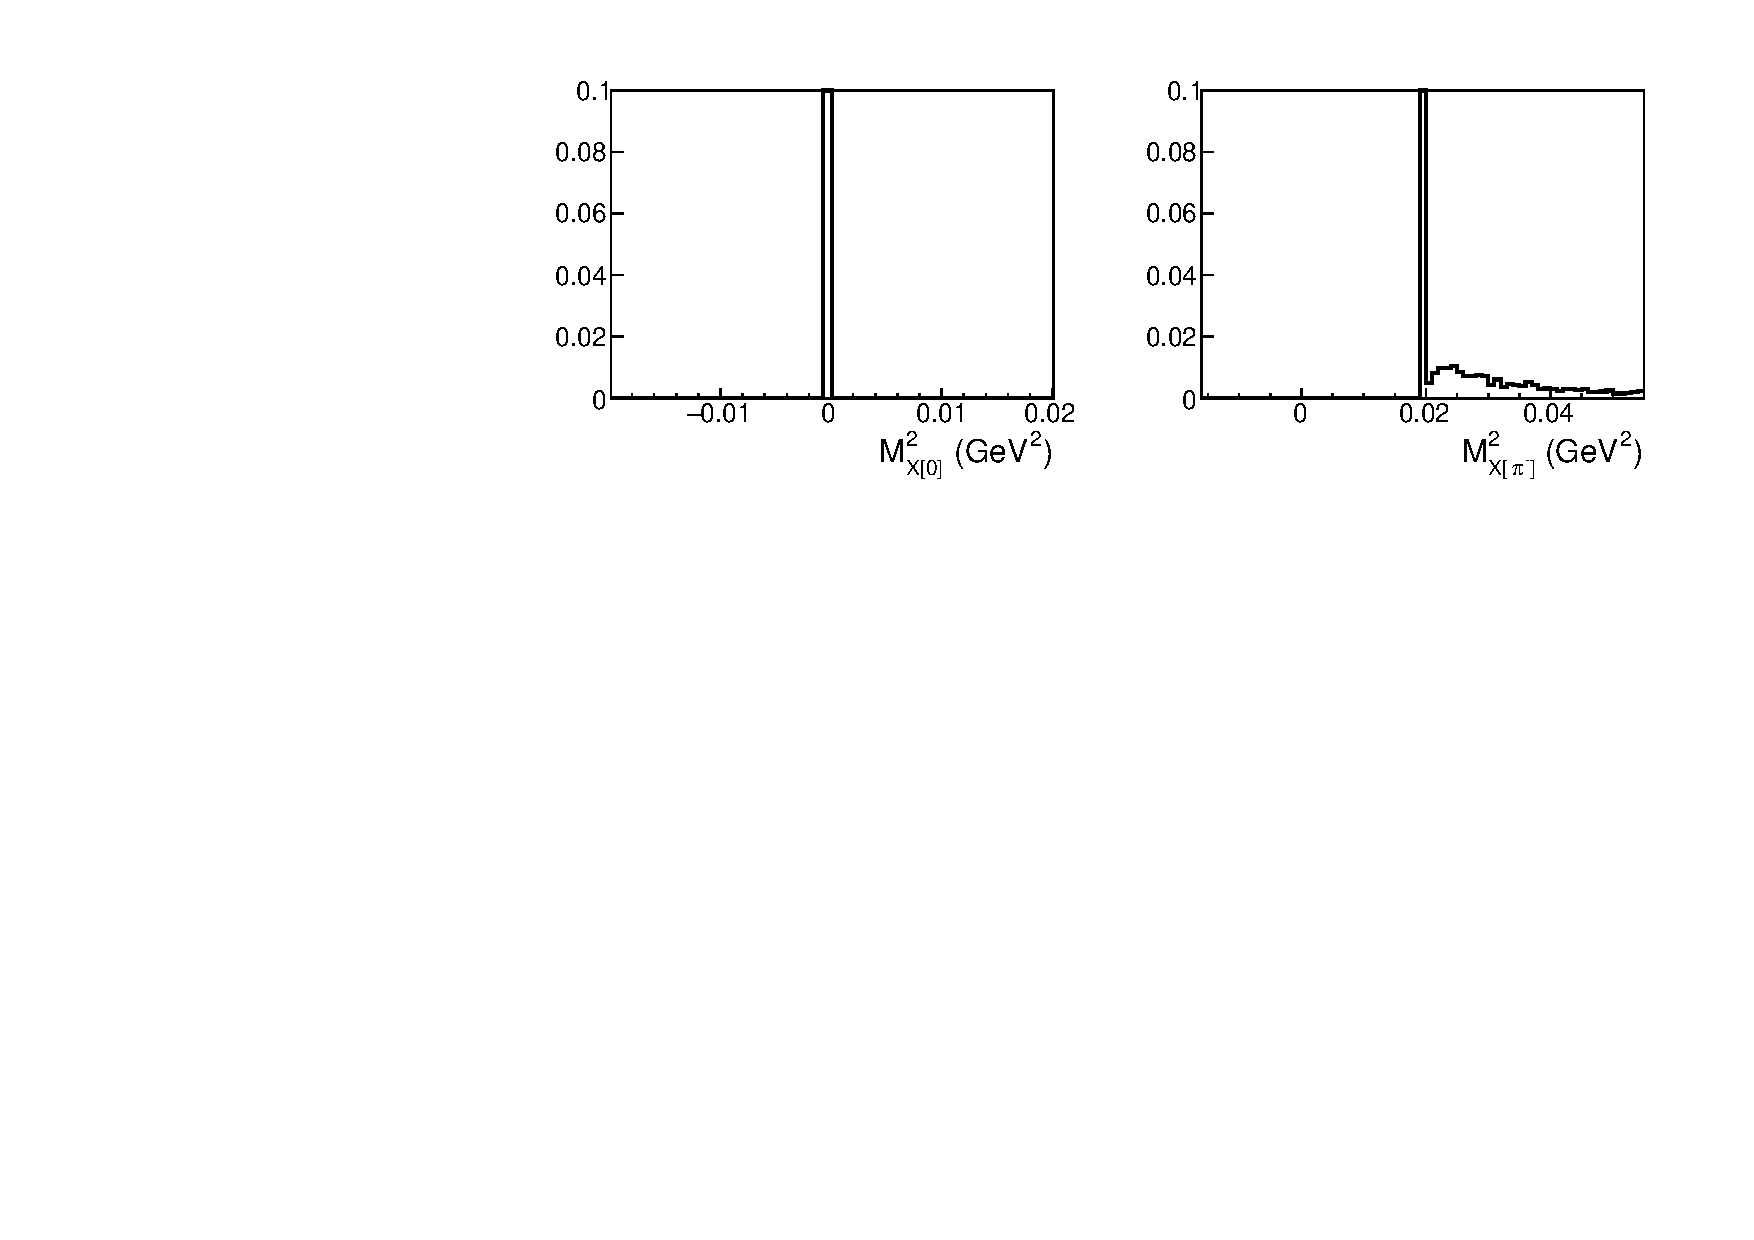
\includegraphics[width=\textwidth]{pictures/mm_rad_nofsi.pdf}}
\caption{\small Impact of radiative effects on $M_{X[0]}^{2}$ (left) and $M_{X[\pi^{-}]}^{2}$ (right). Both distributions are zoomed in on small $y$ to make the impact of radiative effects visible.} \label{fig:mm_rad}
\end{center}
\end{figure}

As follows from Eqs.~\eqref{eq:mm_rad}, the quantity $M_{X[0]}^{2}$ feels no impact of radiative photon emissions as radiated events turn out to contribute to the main distribution peak at zero. Meanwhile, in the distribution of $M_{X[\pi^{-}]}^{2}$, the main peak at $m_{\pi^{-}}^{2}$ acquires a right-side tail, populated with events with photon emissions. This situation is illustrated in Fig.~\ref{fig:mm_rad}, which shows the distributions of $M_{X[0]}^{2}$ (left) and $M_{X[\pi^{-}]}^{2}$ (right) plotted for the event sample affected by radiative effects\footnote[3]{The TWOPEG event generator~\cite{twopeg}, which was used to produce these histograms, employs radiative effects according to the well-known approach from Ref.~\cite{Mo:1968cg}. The minimal photon energy was set to 10~MeV.}.

Note that for the quantity $M_{X[0]}^{2}$ the missing four-vector $P_{X[0]}^{\mu}$ in Eqs.~\eqref{eq:mm_rad} turns out to be the four-momentum of the radiative photon, which is not equal to zero componentwise. However, being massless, the photon has the energy equal to its momentum magnitude, which gives zero upon the calculation of $M_{X[0]}^{2}$. Thus, the zero value of $M_{X[0]}^{2}$ has a different nature for events with and without radiative effects.


